\documentclass[tikz,border=10pt]{standalone}
\usepackage{tikz}
\usetikzlibrary{positioning, arrows.meta}

\begin{document}
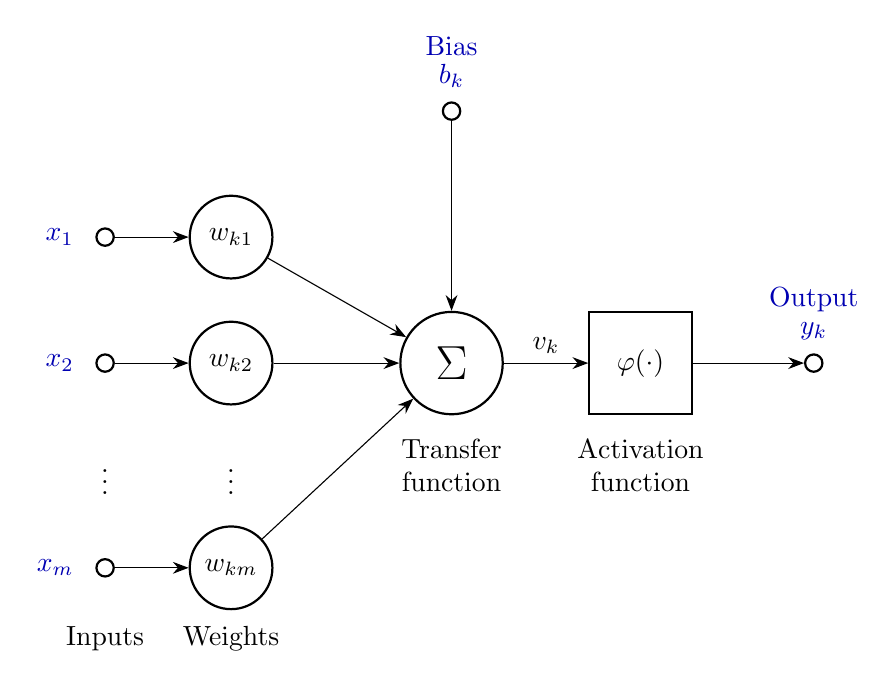
\begin{tikzpicture}[
    >={Stealth[length=2mm]},
    terminal/.style = {circle, draw=black, thick, fill=white, minimum size=0.22cm, inner sep=0pt},
    wnode/.style    = {circle, draw=black, thick, minimum size=1.05cm},
    sumnode/.style  = {circle, draw=black, thick, minimum size=1.3cm, font=\LARGE},
    actnode/.style  = {rectangle, draw=black, thick, minimum size=1.3cm},
    blue/.style     = {text=blue!70!black},
]

% input terminals
\node[terminal] (x1) at (0, 0)    {};
\node[terminal] (x2) at (0, -1.6) {};
\node[terminal] (xm) at (0, -4.2) {};
\node[blue, left=0.15cm of x1] {$x_1$};
\node[blue, left=0.15cm of x2] {$x_2$};
\node[blue, left=0.15cm of xm] {$x_m$};
\node at (0, -3.0) {$\vdots$};

% bias terminal, centered above the summing junction
\node[terminal] (bias) at (4.4, 1.6) {};
\node[blue, above=0.05cm of bias, align=center] {Bias\\[-2pt]$b_k$};

% weight nodes
\node[wnode] (wk1) at (1.6, 0)    {$w_{k1}$};
\node[wnode] (wk2) at (1.6, -1.6) {$w_{k2}$};
\node[wnode] (wkm) at (1.6, -4.2) {$w_{km}$};
\node at (1.6, -3.0) {$\vdots$};

% summing junction
\node[sumnode] (sum) at (4.4, -1.6) {$\Sigma$};

% activation function box
\node[actnode] (act) at (6.8, -1.6) {$\varphi(\cdot)$};

% output terminal
\node[terminal] (yout) at (9.0, -1.6) {};
\node[blue, above=0.05cm of yout, align=center] {Output\\[-2pt]$y_k$};

% edges: inputs -> weights
\draw[->] (x1) -- (wk1);
\draw[->] (x2) -- (wk2);
\draw[->] (xm) -- (wkm);

% edges: weights -> sum, bias -> sum
\draw[->] (wk1) -- (sum);
\draw[->] (wk2) -- (sum);
\draw[->] (wkm) -- (sum);
\draw[->] (bias) -- (sum);

% sum -> activation -> output
\draw[->] (sum) -- (act) node[midway, above] {$v_k$};
\draw[->] (act) -- (yout);

% captions below
\node[align=center] at (0, -5.1) {Inputs};
\node[align=center] at (1.6, -5.1) {Weights};
\node[align=center] at (4.4, -2.9) {Transfer\\function};
\node[align=center] at (6.8, -2.9) {Activation\\function};

\end{tikzpicture}
\end{document}
